\documentclass[10pt]{article}

\def\Type{LessonDJ}
\def\TypeNum{Workshop Week 14} %Lesson #
\def\TypeTitle{Continuous Probability} %Lesson Title
\def\Semester{Fall 2021} %Not Used 
\def\Course{MATH 1190}%Course number and name
\def\Targets{\target{P1}, \target{P2}  }

\usepackage{preambleDJ} 

%%%%%%%%%%%% BEGIN DOCUMENT %%%%%%%%%%%%%%%
%%%%%%%%%%%% BEGIN DOCUMENT %%%%%%%%%%%%%%%
%%%%%%%%%%%% BEGIN DOCUMENT %%%%%%%%%%%%%%%
%%%%%%%%%%%% BEGIN DOCUMENT %%%%%%%%%%%%%%%
%%%%%%%%%%%% BEGIN DOCUMENT %%%%%%%%%%%%%%%

\begin{document}
\pagestyle{otherpages}
\thispagestyle{firstpage}


\vs{.6}

\section{Warm-Up}
Consider the continuous random variable $X$ with the following probability density function p(x) and it's graph:\\
\mpageT{.5}{.5}{\centering
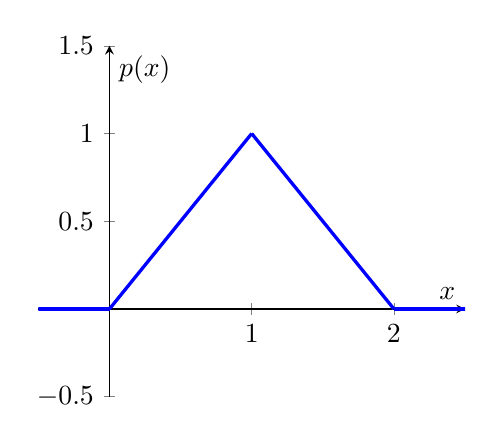
\begin{tikzpicture}
\begin{axis}[
    axis lines = middle,
    xlabel = $x$,
    ylabel = $p(x)$,
    xmin = -0.5, xmax = 2.5,
    ymin = -0.5, ymax = 1.5,
    samples = 200,
    domain = -0.5:2.5,
    width=7cm,
]
% f(x)=x on [0,1]
\addplot[very thick, blue, domain=0:1] {x};
% f(x)=2-x on [1,2]
\addplot[very thick, blue, domain=1:2] {2 - x};
% f(x)=0 elsewhere: left part
\addplot[very thick, blue, domain=-0.5:0] {0};
% right part
\addplot[very thick, blue, domain=2:2.5] {0};
\end{axis}
\end{tikzpicture}
}{
\[
p(x) =
\begin{cases}
0 & x < 0, \\[6pt]
x & 0 \le x \le 1, \\[6pt]
2 - x & 1 \le x \le 2, \\[6pt]
0 & x > 2.
\end{cases}
\]
}
\begin{enumerate}
\item Check that it is truly a probability density function, which means that you have to check the two defining properties.
\item Compute $P(X \leq 0)$, $P(X \leq 0.5)$, $P(X \geq 1)$, $\ds P(X=1/3)$;
\item Find an interval $[0,b]$ where $P(0\leq X \leq b)=7/8$  
\end{enumerate}



\newpage
\section{Expected value and variance (discrete)}
Recall that in the discrete case the expected value (or mean) and the variance are defined as
\[
\mu=E[X]=\sum_{i=1}^nx_i \cdot p(x_i)
\]
\[
Var(X)= \sum_{i=1}^n (x_i-\mu)^2\cdot p(x_i)=  \left( \sum_{i=1}^n x_i^2\cdot p(x_i)  \right) -\mu^2
\]
The histogram below represents the PDF of a random variable $X$. 
\\ 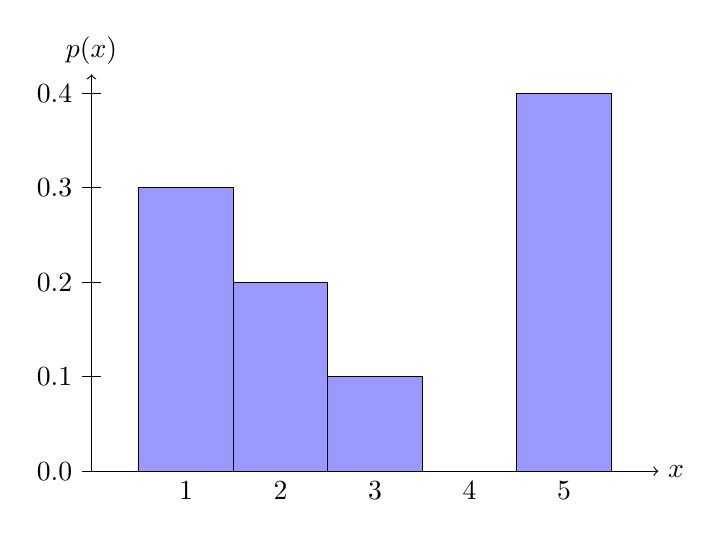
\begin{tikzpicture}[scale=1.2]

    % Axes
    \draw[->] (0,0) -- (6,0) node[right] {$x$};
    \draw[->] (0,0) -- (0,4.2) node[above] {$p(x)$};

    % Y-axis labels
    \foreach \y in {0,1,2,3,4} {
        \draw (-0.1,\y) -- (0.1,\y);     % small tick
        \node[left] at (-0.1,\y) {0.\y};
    }

    % Bars (heights example)
    \draw[fill=blue!40] (0.5,0) rectangle (1.5,3);
    \draw[fill=blue!40] (1.5,0) rectangle (2.5,2);
    \draw[fill=blue!40] (2.5,0) rectangle (3.5,1);
    \draw[fill=blue!40] (3.5,0) rectangle (4.5,0);
    \draw[fill=blue!40] (4.5,0) rectangle (5.5,4);

    % X-axis labels
    \foreach \i in {1,...,5} {
        \node at (\i, -0.2) {\i};
    }

\end{tikzpicture}
\\
\begin{enumerate}
    \item Before computing anything, do you think $X$ has a high variance or a low variance? 
    \item Compute the expected value of $X$;
    \item Compute the variance of $X$;
    \item How would you modify $X$ to lower its mean? sketch the histogram of your suggested modification and compute its mean (remember that the total probability must always be 1);
    \item How would you modify $X$ to increase its variance? sketch the histogram of your suggested modification and compute its variance  (remember that the total probability must always be 1).
\end{enumerate}



\newpage
\section{Expected Value and Variance (continuous)}
Recall that in the continuous case the expected value (or mean) and the variance are defined as
\[
\mu=E[X]=\int_a^b x \cdot p(x) dx
\]
\[
Var(X)=\int_a^b(x-\mu)^2 \cdot p(x) dx=\left( \int_a^b x^2 \cdot p(x) dx \right) -\mu^2
\]
Let $X$ be a continuous random variable with density
\[
p(x)=\frac{3}{4}x(2-x) \qquad \text{for} \quad  0 \leq x \leq 2
\]
and $p(x)=0$ otherwise.
\begin{enumerate}
    \item Check that it is truly a probability density function, which means that you have to check the two defining properties.
    \item Compute the expected value $E[X]$;
    \item Compute the variance $Var(X)$;
\end{enumerate}

\newpage 
\section{Cumulative distribution function}
Consider the continuous random variable from exercise 1, which had probability density function:
\\ 
\mpageT{.5}{.5}{\centering
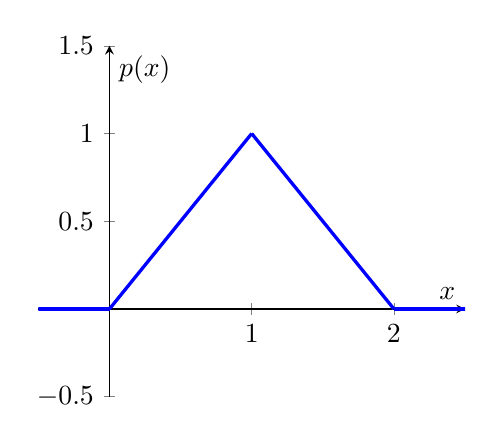
\begin{tikzpicture}
\begin{axis}[
    axis lines = middle,
    xlabel = $x$,
    ylabel = $p(x)$,
    xmin = -0.5, xmax = 2.5,
    ymin = -0.5, ymax = 1.5,
    samples = 200,
    domain = -0.5:2.5,
    width=7cm,
]
% f(x)=x on [0,1]
\addplot[very thick, blue, domain=0:1] {x};
% f(x)=2-x on [1,2]
\addplot[very thick, blue, domain=1:2] {2 - x};
% f(x)=0 elsewhere: left part
\addplot[very thick, blue, domain=-0.5:0] {0};
% right part
\addplot[very thick, blue, domain=2:2.5] {0};
\end{axis}
\end{tikzpicture}
}{
\[
p(x) =
\begin{cases}
0 & x < 0, \\[6pt]
x & 0 \le x \le 1, \\[6pt]
2 - x & 1 \le x \le 2, \\[6pt]
0 & x > 2.
\end{cases}
\]
}

\begin{enumerate}
    \item  Find the corresponding cumulative distribution function, $F(x)$ using steps a), b) and c) below Since $p(x)$ is a piecewise function, $F(x)$ will also be piecewise.
   \[
F(x) =
\begin{cases}
0 & x < 0, \\[6pt]
F_1(x) & 0 \le x \le 1, \\[6pt]
F_2(x) & 1 \le x \le 2, \\[6pt]
1 & x > 2.
\end{cases} 
     \]
    \enum{
    \item Find the cumulative distribution function over the interval $0\leq x\leq 1$. Let's call this $F_1(x)$
    \item Find the cumulative distribution function over the interval $1\leq x\leq 2$. Let's call this $F_2(x)$
    \item Check two things: Is $F_1(1)=F_2(1)$? Is $F_2(2)=1$? If one/both are not true, you probably forgot to add something to the function $F_2(x)$.
    }
    \item Now graph this cumulative distribution function;
    \item Use the cumulative distribution function to find the probability of $P(X \leq 1)$ and $P(X \in [0,1.5])$
    \item  Use the cumulative distribution function to find an interval $[c,1]$ where $P(c\leq X\leq 1)=1/8$.
\end{enumerate}

\end{document}